\section{Praktická časť}
\noindent

Praktická časť tejto diplomovej práce sa zaoberá spojením opisovaných častí do jednej softvérovej knižnice pre platformu Arduino Mega 2560. Arduino využíva AVR
architektúru mikrokontrolérov, preto sme značnú časť práce venovali práve štúdiu fungovania týchto mikrokontrolérov.
Jednou z hlavných úloch vytvorenej knižnice je zjednodušenie použitia prerušení s dôrazom na prerušenia časovačov.
Druhou úlohou je umožnenie vývoja aplikácii mikrokontroléra pomocou udalosťami riadeného programovania. Tento spôsob programovania sme modelovali použitím stavových
automatov. Spojením týchto dvoch fenoménov sme sa pokúsili zjednodušiť a zrýchliť vývoj aplikácii aktívne využívajúcich prerušenia mikrokontroléra.
V predstavených riešeniach je možné program modelovať pomocou udalosťami riadeného programovania,
avšak žiadne z nich neponúka priamu integráciu s prerušovacím systémom mikrokontrolérov. Udalosti v nich sú generované softvérovo. Naše riešenie má za cieľ rovnaké
modelovanie programu pomocou stavových automatov s možnosťou generovania udalostí na softvérovej úrovni. Navyše by však malo umožňovať generovanie udalostí pomocou
prerušení. Knižnica by mala umožniť využitie  prerušení aj menej zdatným používateľom, keďže jej využitie by nemalo vyžadovať hĺbkové znalosti fungovania prerušení na mikrokontroléri Arduino Mega 2560.
Knižnicu sme nazvali Interro a tento názov budeme používať aj neskôr v tejto práci pri opise fungovania a architektúry vytvorenej knižnice. Knižnica je zapísaná v jazyku C++.

\subsection{Predstavenie riešenia}
\noindent
Pre jednoduchšie porozumenie si vytvorenú knižnicu predstavíme na nasledujúcom jednoduchom príklade: Vytvoríme program, ktorého úlohou je blikanie led žiarovky.
Tá bude meniť svoj stav v 1 sekundovom intervale. Blikanie led žiarovky je možné vypnúť, respektíve zapnúť pomocou stlačenia tlačidla.

\subsubsection{Modelovanie programu pomocou stavového automatu}
\noindent
Prvým krokom každého programu vytvoreného pomocou knižnice Interro je jeho namodelovanie pomocou stavového automatu.
Ako sme spomínali v kapitovale číslo \ref{state-machine-theory}, automat je definovaný päticou ($\Sigma$ ,$\mathcal{Q}$ , $q_0$, $\mathcal{F}$, $\delta$).
Automat označíme ako \textit{P} a začneme definíciou množiny stavov $\mathcal{Q}$. V našom príklade vieme identifikovať 3 stavy:
\begin{enumerate}
    \item Led žiarovka svieti, označme ako \textit{LedOn}.
    \item Led žiarovka nesvieti, označme ako \textit{LedOff}.
    \item Blikanie led žiarovky je vypnuté, označme ako \textit{Idle}.
\end{enumerate}

Pokračujme definíciou vstupnej abecedy $\Sigma$. Túto vstupnú abecedu Interro označuje ako udalosti. V spomínanom príklade je možné definovať tieto udalosti:
\begin{enumerate}
    \item Stlačenie tlačidla, označme ako \textit{ButtonClicked}.
    \item Vypršanie časového intervalu, označme ako \textit{TimeElapsed}.
\end{enumerate}

Nasleduje definícia počiatočného stavu $q_0$. Tým je stav \textit{Idle}. Množina konečných stavov $\mathcal{F}$ je v našom prípade prázdna. Príklad nedefinuje
stav v ktorom má program skončiť a už ďalej nepokračovať vo svojej činnosti. K úplnej definícii automatu nám ešte chýba definícia prechodovej funkcie $\delta$.
Tú definujeme pomocou obrázku číslo \ref{figure:blinking-led-state-machine}.

\begin{figure}[!h]
    \centering
    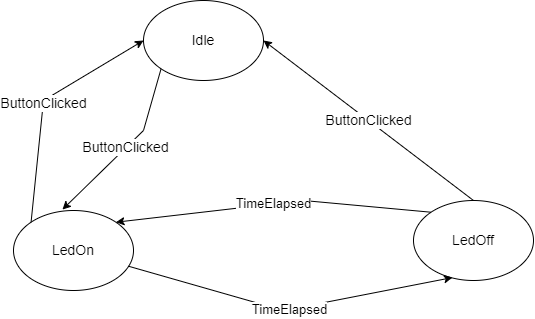
\includegraphics[width=0.85\textwidth]{img/blinking-led-state-machine.png}
    \caption{Stavový automat pre blikajúcu led žiarovku s možnosťou vypnutia pomocou tlačidla}
    \label{figure:blinking-led-state-machine}
\end{figure}

Stavový automat \textit{P} je teda definovaný ako pätica ($\Sigma$ ,$\mathcal{Q}$ , $q_0$, $\mathcal{F}$, $\delta$)
\begin{itemize}
    \item \begin{math} \Sigma = \{ \textit{ButtonClicked}, \textit{TimeElapsed} \}  \end{math}
    \item \begin{math} Q = \{ \textit{LedOn}, \textit{LedOff}, \textit{Idle} \}  \end{math}
    \item \begin{math} q_0 = \{ \textit{Idle} \}  \end{math}
    \item $\mathcal{F}$ \begin{math} = \{ \}  \end{math}
\end{itemize}
a prechodová funkcia $\delta$ je daná obrázkom \ref{figure:blinking-led-state-machine}.

\subsubsection{Implementácia stavového automatu}
Implementáciu začneme vytvorením niekoľkých globálnych premenných. Ako prvé definujeme enum stavov a enum udalostí definovaných v stavovom automate \textit{P}.
\begin{lstlisting}[
    label={lst:events-and-states},
    language=c++]  

enum States
{
    LedOn,
    LedOff,
    Idle
};

enum Events
{
    ButtonClicked,
    TimeElapsed,
};    

\end{lstlisting}
Interro definuje triedu \textit{StateMachine}. Pomocou tejto triedy vieme reprenzentovať stavový automat \textit{P} v našom programe. Trieda definuje jeden
parametrický konštruktor, ktorého argumentom je počiatočný stav automatu. Podľa definície \textit{P} to je stav \textit{Idle}. Vytvoríme preto inštanciu danej triedy s
názvom \textit{blinkingMachine} a nastavíme správny počiatočný stav automatu.
\begin{lstlisting}[
    label={lst:events-and-states},
    language=c++]  

StateMachine blinkingMachine(States::Idle);

\end{lstlisting}

Nasleduje definícia prechodovej funkcie automatu. V knižnici Interro sa prechodová funkcia definuje samostatne pre každý stav.
Definícia pre stav \textit{LedOn} vyzerá nasledovne:

\begin{lstlisting}[language=c++]  

static const int8_t ledOnStateTable[]{
    Events::ButtonClicked, States::Idle,
    Events::TimeElapsed, States::LedOff,
    -1};
    
\end{lstlisting}

Definícia je jednorozmerné pole, ktoré sa skladá z dvojíc udalostí a stavov. Táto dvojica reprezentuje prechod medzi stavmi. V prechodovej funkcii na obrázku číslo
\ref{figure:blinking-led-state-machine} vidíme, že zo stavu \textit{LedOn} sa vieme dostať do stavu \textit{Idle} ale aj do stavu \textit{LedOff}.
To aký bude ďalší stav definuje udalosť (vstupná abeceda), ktorá nastala. To vidíme aj v prechodovej tabuľke: Udalosť \textit{ButtonClicked} hovorí o prechode do stavu
\textit{Idle} a udalosť \textit{TimeElapsed} definuje prechod do stavu \textit{LedOff}. Pre čitateľnosť kódu je dôležité zvoliť správne formátovanie zápisu poľa.
Prechodová tabuľka stavu musí byť vždy ukončená číslom -1. Na základe toho implementácia Interro knižnice zistí veľkosť poľa a je schopná s ním vykonávať operácie.
Rovnakým spôsobom nadefinujeme prechodové tabuľky pre každý stav automatu \textit{P}:

\begin{lstlisting}[language=c++]  

static const int8_t idleStateTable[]{
    Events::ButtonClicked, States::LedOn,
    -1};

static const int8_t ledOnStateTable[]{
    Events::ButtonClicked, States::Idle,
    Events::TimeElapsed, States::LedOff,
    -1};

static const int8_t ledOffStateTable[]{
    Events::ButtonClicked, States::Idle,
    Events::TimeElapsed, States::LedOn,
    -1};
    
\end{lstlisting}

Definovali sme teda stavy, ktoré môže automat nadobudnúť. Rovnako aj udalosti spolu s prechodovými tabuľkami automatu.
Tu ukončíme definíciu globálnych premenných a pokračujeme v implementácii v Arduino funkcii setup(), ktorá je zavolaná jedenkrát pri štarte programu.
Pomocou definovaných globálnych premenných nakonfigurujeme spomínanú premennú \textit{blinkingMachine} typu \textit{StateMachine}. Konfigurácia funguje
na rovnakom princípe ako definícia prechodových tabuliek: každý stav automatu konfigurujeme samostatne. Konfigurácia pre náš príklad je nasledujúca:

\begin{lstlisting}[language=c++]  

blinkingMachine.configure(States::Idle)
    .onEvent(idleStateTable);

blinkingMachine.configure(States::LedOn)
    .onEvent(ledOnStateTable)
    .onEntry([](int8_t state)
            {
                TurnOnLed();
            });

blinkingMachine.configure(States::LedOff)
    .onEvent(ledOffStateTable)
    .onEntry([](int8_t state)
            { 
                TurnOffLed();
            });
        
    \end{lstlisting}

Ako prvé je vždy nutné zavolať metódu \textit{configure} (tento princíp sa opakuje v celej knižnici Interro).
Ako argument do metódy posielame stav, pre ktorý chceme konfiguráciu vykonať. Nasleduje volanie metódy \textit{onEvent}, tu ako argument posielame prechodovú tabuľku
stavu, ktorý konfigurujeme. Po volaní týchto dvoch metód je konfigurácie stavu hotová. Interro nám však umožnuje aj volanie vlastných metód pri vstupe a
výstupe zo stavu. V príklade vidíme volanie metódy  \textit{onEntry}. Do nej je možné poslať smerník na funkciu, prípadne lambda funckiu ako to vidíme
v príklade vyššie. Táto funkcia bude následne zavolaná vždy pri vstupe stavového automatu do konfigurovaného stavu. V našom príklade pri vstupe do stavu
\textit{LedOn} zavoláme funckiu \textit{TurnOnLed}, ktorá zasvieti led žiarovku. Analogicky pri vstupe do stavu \textit{LedOff}, voláme funckiu \textit{TurnOffLed},
ktorá led žiarovku zhasne. Rovnakým spôsobom funguje aj volanie metódy
\textit{onExit}. Jediným rozdielom je, že poskytnutá funkcia bude zavolaná pred opustením daného stavu. Túto možnosť však v našom príklade nevyužívame.

\subsubsection{Spúšťače udalostí}
V predchádzajúcej podkapitole sme namodelovali náš program pomocou stavového automatu a následne sme tento automat pomocou knižnice Interro aj implementovali.
Automat definuje stavy v ktorých sa môže nachádzať. Zároveň definuje aj prechody medzi stavmi a umožnuje volanie vlastných metód užívateľa pri zmene aktuálneho stavu.
Poslednou chýbajúcou časťou sú udalosti a ich spúšťanie. O to sa v Interro knižnici starajú takzvané spúšťače. \par
Spúšťače sú zodpovedné za sledovanie udalostí a ich následnú propagáciu do stavových automatov Interra.
Príkladom spúšťača je \textit{Timer1Trigger}. Využíva časovač číslo 1 mikrokontroléra Arduino Mega 2560 a podporuje rôzné módy.
Práve tento spúšťač použijeme na generovanie udalosti \textit{TimeElapsed}. Prvým krokom je vytvorenie ďalšej globálnej premennej typu \textit{Timer1Trigger}.
Pomenujeme ju ako \textit{timerTrigger}.
\begin{lstlisting}[language=c++]  
Timer1Trigger timerTrigger;            
\end{lstlisting}

Nasleduje konfigurácia spúšťača v Arduino funkcii setup:
\begin{lstlisting}[language=c++]  
timerTrigger.configure(TimerMode::CTC)
    .useInterval(1000, Events::TimeElapsed); 
\end{lstlisting}

Daným kódom konfigurujeme spúšťač, v našom konkrétnom prípade časovač 1, aby používal CTC mód, a po uplynutí každých 1000 milisekúnd oboznámil stavové automaty
o udalosti \textit{TimeElapsed}. Týmto spôsobom zabezpečíme generovanie udalosti \textit{TimeElapsed} každú sekundu. Ná základe tejto udalosti bude stavový automat
prechádzať zo stavu \textit{LedOn} do stavu \textit{LedOff}, respektíve, to isté bude platiť aj opačným smerom. Dôsledkom týchto zmien stavu bude volanie funkcií
\textit{TurnOnLed} respektíve \textit{TurnOffLed}, ktoré zabezpečia blikanie led žiarovky v 1 sekundovom intervale.  \par

Na generovanie udalosti \textit{ButtonClicked} využijeme spúšťač nazvaný ako \textit{ButtonTrigger}. Ako aj v predošlých prípadoch, prvým krokom je definovanie globálnej premennej
\textit{buttonTrigger} typu \textit{ButtonTrigger}.

\begin{lstlisting}[language=c++]  
ButtonTrigger buttonTrigger;            
\end{lstlisting}

Nasleduje konfigurácia spúšťača v Arduino funkcii setup:
\begin{lstlisting}[language=c++]  
buttonTrigger.configure(5)
    .onClick(Events::ButtonClicked); 
\end{lstlisting}

Spúšťač \textit{buttonTrigger} sme nakonfigurovali tak aby sledoval Arduino pin číslo 5 a v prípade stlačenia tlačidla pripojeného na tento pin, vygeneroval udalosť
\textit{ButtonClicked}. Po jej vygenerovaní automat prejde do  \textit{Idle} a blikanie led žiarovky sa zastaví. Po opakovanom stlačení tlačidla automat prejde do
stavu \textit{LedOn} a blikanie led žiarovky sa znovu spustí. \par
Pre správnu funkčnosť celej knižnice je nakoniec nutné v Arduino funkcii \textit{loop} volať metódu \textit{run}, definovanú v globálnom kontajneri Interro knižnice.
\begin{lstlisting}[language=c++]  
void loop()
{
    interro.run();
}
\end{lstlisting}

Týmto krokom sme dokončili funkčnosť názornej ukážky programu. Celý program je možné nájsť v prílohe \ref{att:A}.

\subsection{Architekúra knižnice Interro} \label{subsection:architecture-interro}
Vďaka výberu jazyka C++ sme pri vývoji sme aktívne využívali princípy objektového orientované programovania. Architekúra Interra pozostáva z mnoho vytvorených tried.
Tie je možné rozdeliť na tri hlavné skupiny: Spúšťače, triedy stavového stroja a triedu Interro.
Postupne sa pozrieme na každú túto skupinu a jej úlohy detailnejšie. \par
\begin{enumerate}
    \item Stavový automat
\end{enumerate}
Medzi triedy stavového stroja môžeme zaradiť triedu \textit{StateMachine} a \textit{StateConfiguration}. Ide implementačne o pomerne jednoduché triedy. Ich úlohou
je reprezentácia stavového automatu a všetkých jeho stavov. Po vygenerovaní udalosti zabezpečujú prechod z jedného stavu do ďalšieho spolu s volaním užívateľských
metód. \par

\begin{enumerate}[resume]
    \item Spúšťače
\end{enumerate}
Spúšťače sú najzložitejšou a najrozsiahlejšou súčasťou knižnice Interro.
Delíme ich na dva druhy: hardvérové a softvérové spúšťače. \par
Hardvérový spúšťač používa na informovanie o udalosti prerušenia mikrokontroléra. Je napojený priamo na ISR prerušenia a obsahuje logiku pre konfiguráciu prerušení,
ktoré podporuje. Knižnica Interro momentálne obsahuje spúšťače pre tieto prerušenia:
\begin{itemize}
    \item Prerušenia časovačov 1, 3, 4 a 5.
    \item Externých prerušení 0 až 7.
    \item Prerušenia hovoriace o zmene hodnoty pinov, takzvané \textit{PinChangeInterrupt} 0 až 3.
\end{itemize}

Každý z týchto spúšťačov má samostatnú triedu a fungujú nezávisle od seba. Preto je možné, respektíve nutné, každý z nich
nakonfigurovať samostatne. Jediným obmedzením je hardvérová implementácia mikrokontroléra. V niektorých prípadoch sú rôzne prerušenia napojené na rovnaký pin procesora,
preto je nutné pre správnu funkčnosť takýmto zhodám predchádzať. \par

Druhým typom spúšťačov sú takzvané softvérove spúšťače. Pri hardvérových spúšťačoch je prvotným impulzom na vygenerovanie udalosti mikrokontrolér. Ten pomocou prerušenia
oboznámi hardvérový spúšťač o novej udalosti. Ak žiadne prerušenie nenastalo, spúšťač nevykonáva žiadnu akciu. Pri softvérových spúšťačoch to funguje inak. Interro knižnica
má zoznam všetkých softvérových spúšťačov a neustále sa na ne dopytuje či niektorá z udalosí nenastala. Ak spúštač odpovie definovanou udalosťou,
tak tá je rovnakým spôsobom preposlaná do všetkých zaregistrovaných stavových automatov. V knižnici Interro je momentálne implementovaný jeden takýto spúšťač s názvom
\textit{ButtonTrigger}. Je možné ho využiť na generovanie udalostí pri stlačení tlačidla. Jeho hlavným cieľom je však demonštrácia rozšíriteľnosti  knižnice o akékoľvek
ďalšie spúšťače. Softvérové spúšťače môžu slúžiť na využitie procesora v čase mimo prerušení. Dopĺňajú tak funkcionalitu Interro knižnice pomocou ktorej je tak
možné vykonávať úlohy na základe vplyvov rôznych periférii (prerušení), ale aj na základe aktálneho stavu programu. \par

\begin{enumerate}[resume]
    \item Globálny kontajner Interro
\end{enumerate}

Trieda Interro slúži ako globálny kontajner a koordinuje činnosť celej knižnice. Pomocou zreťazených zoznamov si ukladá všetky inštancie vytvorených stavových automatov
ale aj hardvérových a softvérových spúšťačov. Počas práce s knižnicou by mala existovať len jedna inštancia tejto triedy. Vytvára ju knižnica a všetky ostatné komponenty
následne pracujú s touto inštanciou triedy Interro. Zabezpečuje fungovanie hardvérových, ako aj softvérových spúšťačov. Vygenerované udalosti následne preposiela do
existujúcich stavových automatov. \par
S triedou Interro úzko súvisí aj trieda \textit{InterruptHandler}. Tá obsahuje ISR pre všetky podporované prerušenia. Ukážku ISR pre overflow prerušenie časovača 1
je možné vidieť nižšie:
\begin{lstlisting}[language=c++]  
#if TIMER1_OVF_INTERRUPT
ISR(TIMER1_OVF_vect)
{
    interro.handleInterrupt(TIMER1_OVF_INTERRUPT_ID);
}
#endif
\end{lstlisting}


Vidíme, že podmienkou kompilácie danej ISR je expanzia makra \\ \textit{TIMER1\_OVF\_INTERRUPT} na logickú jednotku. Makro je definované v hlavičkovom súbore triedy Interro.
Táto podmienená kompilácia je dostupná pre pokročilých užívateľov knižnice. Každý program môže obsahovať len jednu definúciu ISR pre každý vektor prerušenia. Preto je
možné v hlavičkovom súbore prepísať expanziu makra \textit{TIMER1\_OVF\_INTERRUPT} na logickú 0 a odstrániť ho z kompilácie v Interro knižnici. Vďaka tomu užívateľ získa
možnosť definovania ISR nezávisle od knižnice Interro. V ISR prerušenia sa nachádza volanie metódy \textit{handleInterrupt}, ktorá informáciu o prerušení dristribuuje
do ostatným komponentov knižnice. Prerušenie je identifikované na základe jeho identifikátora. Ten je definovaný v hlavičkovom súbore triedy Interro, a je používaný
ako argument metódy \textit{handleInterrupt}.
Rovnakým spôsobom sú implementované všetky podporované prerušenia knižnice Interro.

\subsubsection{Komunikácia medzi komponentami knižnice Interro}
Komunikáciu s a vrámci knižnice je možné rozdeliť do dvoch fáz. \par
Prvá fáza je konfiguračná a prebieha okamžite po spustení programu. Jej obsahom je správne
nastavenie spúšťačov a definícia stavových automatov. Na platforme Arduine prebieha vo funkcii \textit{setup} a je spustená práve jeden krát. V tejto fáze sa knižnica
rôznymi spôsobmi snaží konfiguráciu a nastavenie spúšťačov čo najviac zjednodušiť. Jedným zo spôsobov je implicitné pridávanie použitých komponentov do globálneho
kontajnera knižnice. Vďaka tomu užívateľ nemusí písať veľa „zbytočného“ kódu. Ďalším je dodržiavanie konvencíí v rámci celej knižnice. Jednou z nich je napríklad
volanie metódy \textit{configure}. Akákoľvek konfigurácia, akéhokoľvek komponentu knižnici musí začínať volaním tejto metódy.  \par

Fáza číslo 2 začína okamžite po skončení prvej fázy. V tejto fáze prebieha generovanie  udalostí, zmena stavov automatov a volanie užívateľských funkcií pri prechodoch
medzi stavmi. Udalosť môže byť vygenerovaná buď hardvérovým alebo softvérovým spúšťačom,  preto aj následná komunikácia je určitým spôsobom rozdielna.
Ak bola udalosť vygenerovaná hardvérovým spúšťačom, komunikácia je zobrazená na sekvenčnom diagrame na obrázku číslo \ref{figure:interrupt-trigger}.
Diagram zobrazuje nasledovné procesy:
\begin{enumerate}
    \item Procesor prestane vykonávať aktuálny kód, a spustí ISR daného prerušenia.
    \item ISR definované v triede \textit{InterruptHandler} oboznámi o prerušení triedu \textit{Interro}.
    \item Trieda \textit{Interro} sa následne „opýta“ každého hardvérového spúšťača či je potrebné vygenerovanie novej udalosti. Ak áno, spúšťač odpovie udalosťou, ktorú je potrebné vygenerovať.
    \item Ak spúšťač odpovie nedefinovanou udalosťou, komunikácia sa končí. V opačnom prípade Interro oboznámi o novej udalosti všetky stavové automaty.
    \item Automat sa po oboznámení o udalosti pozrie do svojej aktuálnej stavovej tabuľky. Ak sa v nej nachádza vygenerovaná udalosť, vykoná prechod z jedného stavu do druhého.
          V prípade, že užívateľ zadefinoval funkcie, ktoré chce pri vstupe/výstupe zo stavu volať, zavolajú sa pri tomto procese.
\end{enumerate}

\begin{figure}[!h]
    \centering
    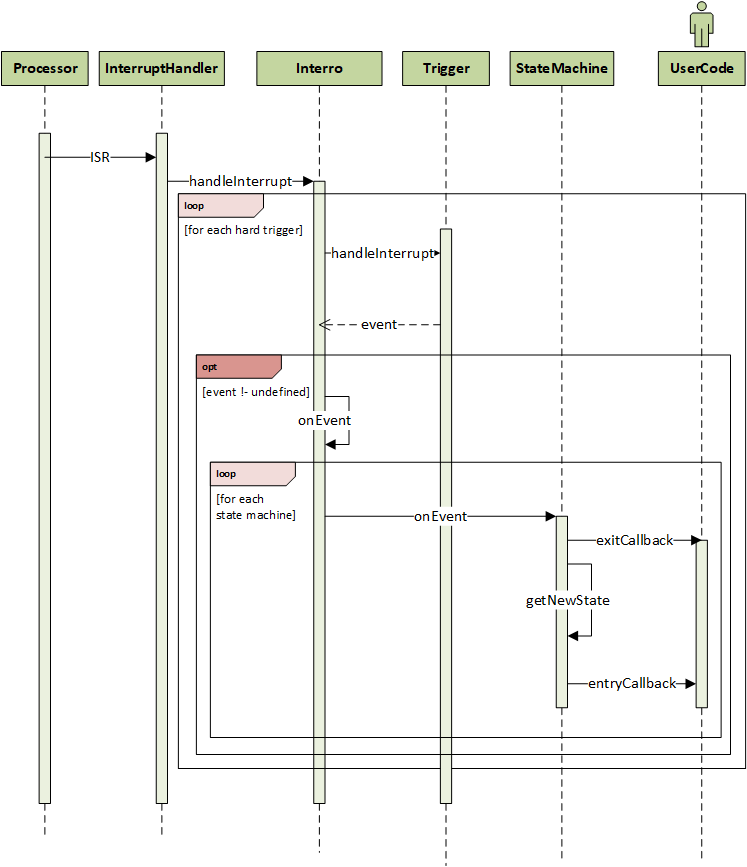
\includegraphics[width=0.95\textwidth]{img/interrupt-sequence.png}
    \caption{Sekvenčný diagram komunikácie pri vygenerovaní udalosti prerušením}
    \label{figure:interrupt-trigger}
\end{figure}



\begin{figure}[!h]
    \centering
    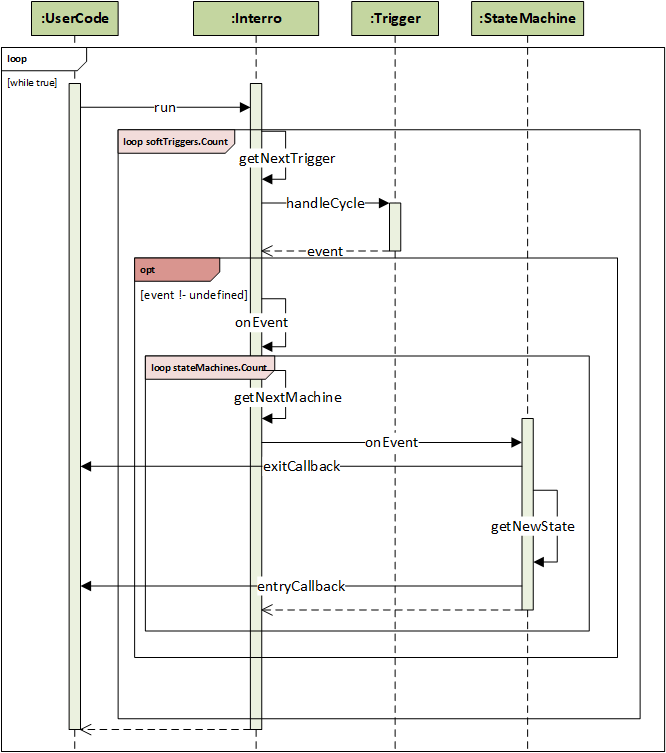
\includegraphics[width=0.95\textwidth]{img/softTrigger-sequence.png}
    \caption{Sekvenčný diagram komunikácie pri vygenerovaní udalosti softvérovým spúšťačom}
    \label{figure:soft-trigger}
\end{figure}


Podobný proces funguje aj pri softvérových prerušeniach. Ten je zobrazený na sekvenčným diagramom na obrázku číslo \ref{figure:soft-trigger}.
Princíp fungovania softvérových spúšťačov je však iný ako v prípade hardvérových. Pre ich správnu funkčnosť je nutné aby bola v užívateľskom kóde neustále
volaná metóda \textit{run} definovaná v triede \textit{Interro}. To zabezpečí cyklenie nižšie popísaného procesu a tým aj správne fungovanie knižnice:

\begin{enumerate}
    \item Intero sa dopytuje na všetky softvérové spúšťače či nastala nejaká udalosť.
    \item Ak spúšťač odpovie nedefinovanou udalosťou, komunikácia sa končí. V opačnom prípade Interro oboznámi o novej udalosti všetky stavové automaty.
    \item Automat sa po oboznámení o udalosti pozrie do svojej aktuálnej stavovej tabuľky. Ak sa v nej nachádza vygenerovaná udalosť, vykoná prechod z jedného stavu do druhého.
          V prípade, že užívateľ zadefinoval funkcie, ktoré chce pri vstupe/výstupe zo stavu volať, zavolajú sa pri tomto procese.
\end{enumerate}

\subsubsection{Implementované spúšťače}

Ako sme spomínali v kapitole číslo \ref{subsection:architecture-interro}, knižnica momentálne implementuje 16 hardvérových spúšťačov troch druhov. Vďaka použitiu
objektovo orientovaného programovania a dedičnosti nebolo nutné každý z týchto spúšťačov implementovať samostatne.
Na ich implementáciu je použitá štruktúra zobrazená na diagrame na obrázku číslo \ref{figure:timer-class-diagram}:
\begin{figure}[!h]
    \centering
    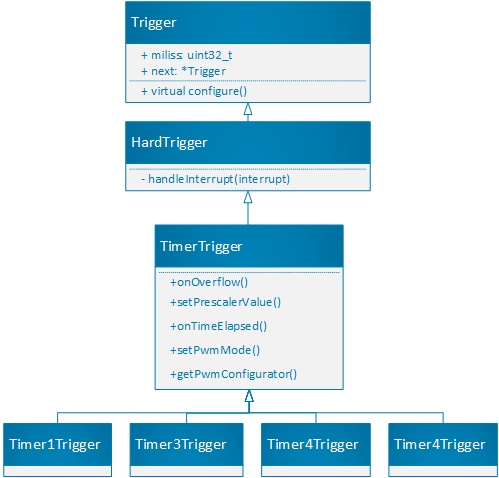
\includegraphics[width=0.95\textwidth]{img/timer-class-diagram.png}
    \caption{Diagram tried pre implementované časové spúšťače}
    \label{figure:timer-class-diagram}
\end{figure}

Všetka logika implementácie a práce s registrami časovača sa nachádza v triede \textit{TimerTrigger}. V nej je definovaný parametrický konštruktor, ktorý
je zavolaný z tried ktoré túto triedu zdedili. Na príklade nižšie vidíme spôsob akým je implementovaný časovač číslo 1. V implementácii sa nachádza len volanie
konštruktora rodiča danej triedy s doplnenými parametrami. Každý z časovačov takýmto spôsobom posiela do triedy \textit{TimerTrigger} adresy na svoje
kontrolné registre, porovnávacie registre, masku prerušení, identifikátory podporovaných prerušení a nakoniec konfiguráciu pre generovanie PWM signálu.

\begin{lstlisting}[language=c++]  

    #include <Timer1Trigger.hpp>

    Timer1Trigger::Timer1Trigger()
        : TimerTrigger(&TCCR1A,
                       &TCCR1B,
                       &TCCR1C,
                       &OCR1A,
                       &OCR1B,
                       &OCR1C,
                       &TIMSK1,
                       TIMER1_OVF_INTERRUPT_ID,
                       TIMER1_COMPA_INTERRUPT_ID,
                       TIMER1_COMPB_INTERRUPT_ID,
                       TIMER1_COMPC_INTERRUPT_ID,
                       TimerPwmConfiguration(1,
                                             &TCCR1A,
                                             PwmPin(&OCR1A, COM1A0, COM1A1),
                                             PwmPin(&OCR1B, COM1B0, COM1B1),
                                             PwmPin(&OCR1C, COM1C0, COM1C1)))
    {
    }
\end{lstlisting}

Na rovnakom princípe je založená implementácia spúšťačov pre zvyšné dva druhy implementovaných spúšťačov. \par

\paragraph*{TimerTrigger} \: je základnou triedou pre implementáciu spúšťačov postavených na 16-bitových časovačoch. Podporuje štandardný mód, CTC mód a PWM mód časovača.

\begin{enumerate}
    \item Normálny mód.
\end{enumerate}

V normálnom móde spúšťač umožnuje generovanie udalosti po pretečení registra časovača. Zároveň je možné manuálne nastaviť hodnotu preddeličky.
Príklad konfigurácie spúštača pre použitie v normálnom móde:
\begin{lstlisting}[language=c++]      
timerTrigger.configure(TimerMode::Normal)
    .onOverflow(Events::TimeElapsed)
    .setPrescalerValue(Prescalers::Prescaler64);
\end{lstlisting}

\begin{enumerate}[resume]
    \item CTC mód
\end{enumerate}

Pri CTC móde je možné definovať až časy pri ktorých bude vygenerovaná nakonfigurovaná udalosť. Pri každom definovanom čase spúšťač automaticky prepočíta
hodnotu preddeličky. Ak sú požadované hodnoty nekompatibilné a hodnotu preddeličky nieje možné násjť, spúšťač program ukončí ešte v jeho 1 fáze. Po ukončení programu
sa spúštač pokúsi poslať dostupné informácie o chybe pomocou sérioveho portu mikrokontroléra. Týmto spôsobom sa knižnica aktívne snaží o zjednodušenie ladenia programu.
Príklad konfigurácie spúštača pre použitie CTC módu s použitím 1 sekundového intervalu, a generovaním udalostí po 80, 600 a 1000 milisekundách:
\begin{lstlisting}[language=c++]      
timerTrigger.configure(TimerMode::CTC)
    .useInterval(1000, Events::Interval1)
    .onTime(600, Events::Interval2)
    .onTime(80, Events::Interval3);
\end{lstlisting}

\begin{enumerate}[resume]
    \item PWM mód
\end{enumerate}

PWM mód slúži na generovanie PWM signálu. Koncepčne vykonáva niečo iné ako spúštač, avšak kvôli jednoduchosti riešenia sme sa rozhodli ho ponechať súčasťou časových
spúštačov. Spúšťač v PWM móde podporuje 6 rôzny PWM módov 16 bitového časovača:
\begin{itemize}
    \item 3 variácie FastPWM módu: 8, 9 a 10 bitová maximálna hodnota registra časovača.
    \item 3 variácie PhaseCorrectPWM módu: 8, 9 a 10 bitová maximálna hodnota registra časovača.
\end{itemize}

Pomocu konfigurácie je možné nastaviť striedu PWM signálu. Spúšťač percentuálne vyjadrenie automaticky prepočíta na hodnotu registra. Rovnakým spôsobom je možné
aj manuálne nastavenie hodnoty registra. Príklad použitia PWM módu so striedou 70\% na  výstupe porovnávacieho registra A je možné vidieť nižšie:

\begin{lstlisting}[language=c++]      
Timer1Trigger timerTrigger;

timerTrigger.configure(TimerMode::PWM)
    .setPwmMode(PwmMode::FastPwm8Bit)
    .setUpOutput(TimerPwmOutput::A, 0.7);
\end{lstlisting}


\paragraph*{ExternalTrigger} \: je základnou triedou pre generovanie udalostí pomocou externých prerušení mikrokontroléra. Je zdedaná triedami ExternalTrigger 0 až 7.
Pri konfigurácii je možné nastaviť stav pri ktorom sa má udalosť vygenerovať. Udalosť je možné generovať ak je stav pinu nízky, ak sa logická hodnota pinu zmenila, prípade
začne stúpať alebo klesať. Pri zmene hodnoty pinu často dochádza k určitému šumu, ktorý môže spôsobiť vygenerovanie viac ako jedného prerušenia v krátkom časovom intervale.
Aby sme takémuto javu predišli, spúštač podporuje nastavenie minimálneho časového intervalu medzi udalosťami.
Štandardná dĺžka intervalu je 300 milisekúnd, avšak používateľovi je umožnené použitie vlastnej hodnoty.
Príklad použitia spúštača pre externé prerušenia je možné vidieť nižšie. Spúšťač je nakonfigurovaný tak, aby pri zmene hodnoty pinu vygeneroval udalosť \textit{PinChanged}.
Minimálny interval medzi udalosťami je 500 milisekúnd.
\begin{lstlisting}[language=c++]      
ExternalTrigger0 externalTrigger0;

externalTrigger0.configure(ExternalTriggerMode::Change)
    .debounce(500)
    .onOccurrence(Events::PinChanged);
\end{lstlisting}

\paragraph*{PinChangeTrigger} \: je základnou triedou pre generovanie udalostí pomocou prerušení o zmene pinu. Je zdedaná triedami \textit{PinChangeTrigger} 0 až 2.
Triedy reprezentujú porty procesora a na každom z nich je možné povoliť pin pre generovanie udalosti. Rovnako ako \textit{ExternalTrigger}, aj \textit{PinChangeTrigger}
podporuje minimálny časový interval medzi dvoma udalosťami. Príklad konfigurácie je možné vidieť nižšie:
\begin{lstlisting}[language=c++]      
PinChangeTrigger0 pinChangeTrigger0;

pinChangeTrigger0.configure()
    .enablePin(1)
    .onOccurrence(Events::PinChanged);
\end{lstlisting}

\paragraph*{ButtonTrigger} \: je implementovaný softvérový spúštač, ktorý pre generovanie udalostí sleduje stav poskytnutého pinu. Funguje na princípe neustáleho
dopytovania sa na aktuálny stav. Po nastavení logickej jednotky na pin, spúštač vygeneruje udalosť. Rovnako ako predošlé spúšťače, podporuje nastavenie minimálneho
časového intervalu medzi dvoma vygenerovanými udalosťami. Cieľom tejto diplomovej práce je generovanie udalostí pomocou prerušení. Preto tento softvérový spúštač
slúži hlavne ako demonštrácia možností rozšírenie knižnice aj o iné spúštače.
Použitie triedy \textit{ButtonTrigger} môžeme vidieť nižšie:

\begin{lstlisting}[language=c++]         
ButtonTrigger buttonTrigger; 

buttonTrigger.configure(5)
    .debounce(500)
    .onClick(Events::ButtonClicked);
\end{lstlisting}

\subsubsection{Rozšíriteľnosť riešenia}

Vyvinuté riešenie nieje obmedzené na už implementované súčasti. Stavový automat podporuje variabilné množstvo stavov a udalostí. Pri modelovaní programu je možné použitie
viacerých stavových automatov, ktoré môžu medzi sebou komunikovať. Pre podporu ďalších prerušení
je možné implementovať ďalšie spúštače. Takýmto spôsobom je možné knižnicu rozšírovať o ďalšie generátory udalostí. Jedinou podmienkou vytvorenia nových spúštačov je
zdedenie triedy \textit{HardTrigger}, respektíve \textit{SofTrigger} a implementovanie náležitých súčasti týchto základných tried.

\subsection{Porovnanie s existujúcimi riešeniami}
Vyvinuté riešenie je možné porovnávať s existujúcimi v dvoch rovinách. Prvou je správa a konfigurácia prerušení, druhou modelovanie programu stavovými automatmi.

\subsubsection{Konfigurácia prerušení}

Žiadne z predstavených riešení nepodporuje konfiguráciu prerušení takým spôsobom akým to umožňuje Interro. Ako príklad uvedieme porovnanie konfigurácie časovača 1 pomocou vytvorenej
knižnice a konfiguráciu časovača manuálnym spôsobom. Ak chceme nakonfigurovať časovač 1 mikrokontroléra Arduino Mega 2560 použitím Interro, dosiahneme to nasledovným spôsobom:

\begin{lstlisting}[language=c++]      
timerTrigger.configure(TimerMode::CTC)
    .useInterval(1000, Events::Interval1);
\end{lstlisting}

Pre porovnanie nižšie vidíme rovnaké nastavenie pomocou kontroloných registrov časovača. Prvým krokom je vynulovanie aktuálnych hodnôt v registroch.
Nasleduje natavenie porovnávacej hodnoty. Na jej výpočet bolo potrebné potrebné použiť vzorec číslo \ref{eq:register-value} spolu so zvolením správnej hodnoty
preddeličky. V posledných dvoch krokoch povolíme CTC mód časovača a následne aj prerušenia pre porovnávací registra A.

\begin{lstlisting}[language=c++]      
    TCCR1A = 0;
    TCCR1B = 0;
    TCCR1C = 0;

    OCR1A = 62499;           // set compare value
    TCCR1B |= (1 << CS12);   // set prescaler to 256
    TCCR1B |= (1 << WGM12);  // enable ctc mode
    TIMSK1 |= (1 << OCIE1A); // enable OCRA interrupt
    
\end{lstlisting}

Na manuálnu konfiguráciu časovača užívateľ potrebuje poznať názvy registrov, názvy jednotlivých bitov  v registroch a model fungovanie časovača ako celku. Pre nadobudnutie
týchto znalosti je nutné štúdium dátového hárku mikrokontroléra. To celý vývoj aplikácie predĺži a spomalí. Použitie viacerých intervalov,
prípadne generovanie  PWM signálu pomocou PWM módu časovača by celú
manuálnu konfiguráciu ešte viac skomplikovalo. Kód je navyše ťažko čitateľný a pre iných programátorov
môže byť nezrozumiteľný. Pri použití vytvorenej knižnice všetky tieto nastavenia registrov vykoná knižnica za užívateľa. \par
Na druhej strane, medzi výhody manuálnej konfigurácie určite patrí väčšia flexibilita riešenia. Časový spúšťač implementovaný v knižnici nepodporuje všetky dostupné
módy a nastavenia, ktoré sú hardvérovo implementované mikrokontrolérom. To pre niektorých pokročilých užívateľov môže byť problém a preto použitie knižnice
v tomto prípade nieje správnym riešením.

\subsubsection{Udalosťami riadené programovanie}
Rovnako ako vyvinutá knižnica, aj existujúce riešenia \textit{Eventually} a \textit{Automaton} podporujú paradigmu udalosťami riadeného programovania. Podľa kapitoly
číslo \ref{section:event-driven-programming} túto paradigmu môžeme rozdeliť na dva druhy: Na programy, ktoré si uchovávajú aktuálny stav a na programy, ktoré nepoznajú
kontext v ktorom udalosť nastala. Interro modeluje program pomocou stavových automatov preto patrí do prvej skupiny spolu s knižnicou Automaton. Do druhej skupiny
zaraďujeme knižnicu Eventually, ktorá nepozná žiaden mechanizmus, ktorým by si uchovávala už vykonané kroky. \par
Na krátkom programe nižšie vidíme použitie knižnice Eventually \cite{bartlettEventually2021}. V príklade blikajúcej led žiarovky môžeme vidieť,
že aktuálny stav žiarovky si je nutné ukladať mimo poskytnutej knižnice. Pri namodelovaní programu pomocou knižnice Interro alebo Automaton
sa zapamätanie aktuálneho stavu zabezpečí už pomocou jeho modelovania ako stavového automatu. Eventually umožňuje len reagovanie na časovú udalosť.
\begin{lstlisting}[language=c++]      
    #include <Eventually.h>       

    #define LIGHT_PIN 5    

    EvtManager mgr;
    bool state = LOW;    

    void setup() {
      pinMode(LIGHT_PIN, OUTPUT);
      mgr.addListener(new EvtTimeListener(1000, true, (EvtAction)blinkme)); 
    }    

    bool blinkme() {
      state = !state; // Switch light states
      digitalWrite(LIGHT_PIN, state); // Display the state
      return false; // Allow the event chain to continue
    }    

    USE_EVENTUALLY_LOOP(mgr) // Use this instead of your loop() function.    
\end{lstlisting}

Základnou operáciou pri udalosťami riadnom programovaní je generovanie udalostí. Existujúce knižnice Automaton a Eventually umožňujú generovanie udalostí pomocou
neustáleho kontrolovania ich stavu. Ak by však nastala niektorá z udalostí a knižnica by v tej chvíli bola zaneprázdnená obsluhou inej činnosti,
mohlo by dôjsť k premeškaniu udalosti. Tento problém sme sa pokúsili vyriešiť v knižnici Interro. Zachovali sme
možnosť generovania udalostí spôsobom akým to robili existujúce riešenia, pridali sme však aj možnosť generovania udalostí pomocou prerušení. Generovanie prerušení pomocou
prináša aj niektoré nevýhody. Prerušenia sú úzko naviazané na procesor, ktorý sme použili pri vývoji. Nieje preto zaručená funkčnosť knižnice aj na iných modeloch
mikrokontrolérov. Nezabraňuje to však použitiu knižnice s použitím
softvérových spúšťačov. Ďalšou z nevýhod je obsluha udalostí. Keďže udalosť bola vygenerovaná pri obsluhe prerušenia, aj obsluha udalosti prebieha vo vnútri prerušenia.
Pri dlho trvajúcej obsluhe udalosti to môže predstavovať problém v podobe premeškania ďalších prichádzajúcich prerušení.
Porovnanie spomínaných knižníc je prehľadne zobrazené v tabuľke číslo \ref{table:library-compare}.
\begin{table}[!htbp]
    \begin{center}
        \begin{tabular}{| m{20em} | c | c | c |}
            \hline
            Funkcionalita                                        & Interro   & Eventually & Automaton \\
            \hline
            Možnosť definovania vlastných udalostí               & Áno       & Áno        & Áno       \\
            \hline
            Uchovávanie aktuálneho stavu programu                & Áno       & Nie        & Áno       \\
            \hline
            Generovanie udalostí pomocou prerušení               & Áno       & Nie        & Nie       \\
            \hline
            Podpora rôznych mikrokontrolérov                     & Čiastočne & Áno        & Áno       \\
            \hline
            Možnosť použitia viac ako jedného stavového automatu & Áno       & -          & Áno       \\
            \hline
            Generovanie PWM signálu pomocou časovačov            & Áno       & -          & -         \\
            \hline
        \end{tabular}
        \caption{Porovnanie knižníc Interro, Eventually a Automaton}
        \label{table:library-compare}
    \end{center}
\end{table}

